\documentclass[unicode,11pt,a4paper,oneside,numbers=endperiod,openany]{scrartcl}

\usepackage{float}
\usepackage{graphicx}
\usepackage[export]{adjustbox}
\usepackage{matlab-prettifier}

\graphicspath{./img/}

\renewcommand{\thesubsection}{\arabic{subsection}}

\input{assignment.sty}
\begin{document}


\setassignment
\setduedate{Wednesday, 8 November 2023, 11:59 PM}

\serieheader{Numerical Computing}
{2023}
{\textbf{Student:} Jeferson Morales Mariciano \\\newline}
{\textbf{Discussed with:} Leonardo Birindelli, Filippo Piloni, Michele Dalle Rive}
{Solution for Project 3}{}
\newline

\assignmentpolicy


\newpage

\subsection{Spectral clustering of non-convex sets [50 points]}

All solutions provided from \textit{ClusterPoints.m}, \textit{epsilonSimGraph.m} source code. \\
A seed for the random number generator has been set $rng(20020309)$, for the results to be replicable.

%--------------------------------------------------------------------------------------
\subsubsection{
    Consider the set named half-kernel: can you identify the two
    obvious clusters in this dataset? Describe them briefly and explain what difficulties a clustering algorithm could
    eventually encounter in a scenario of this kind.}


\begin{figure}[H]
    \centering
    \caption{Halfkernel non-convex set}
    \label{fig:ex1-1-halfkernel}
    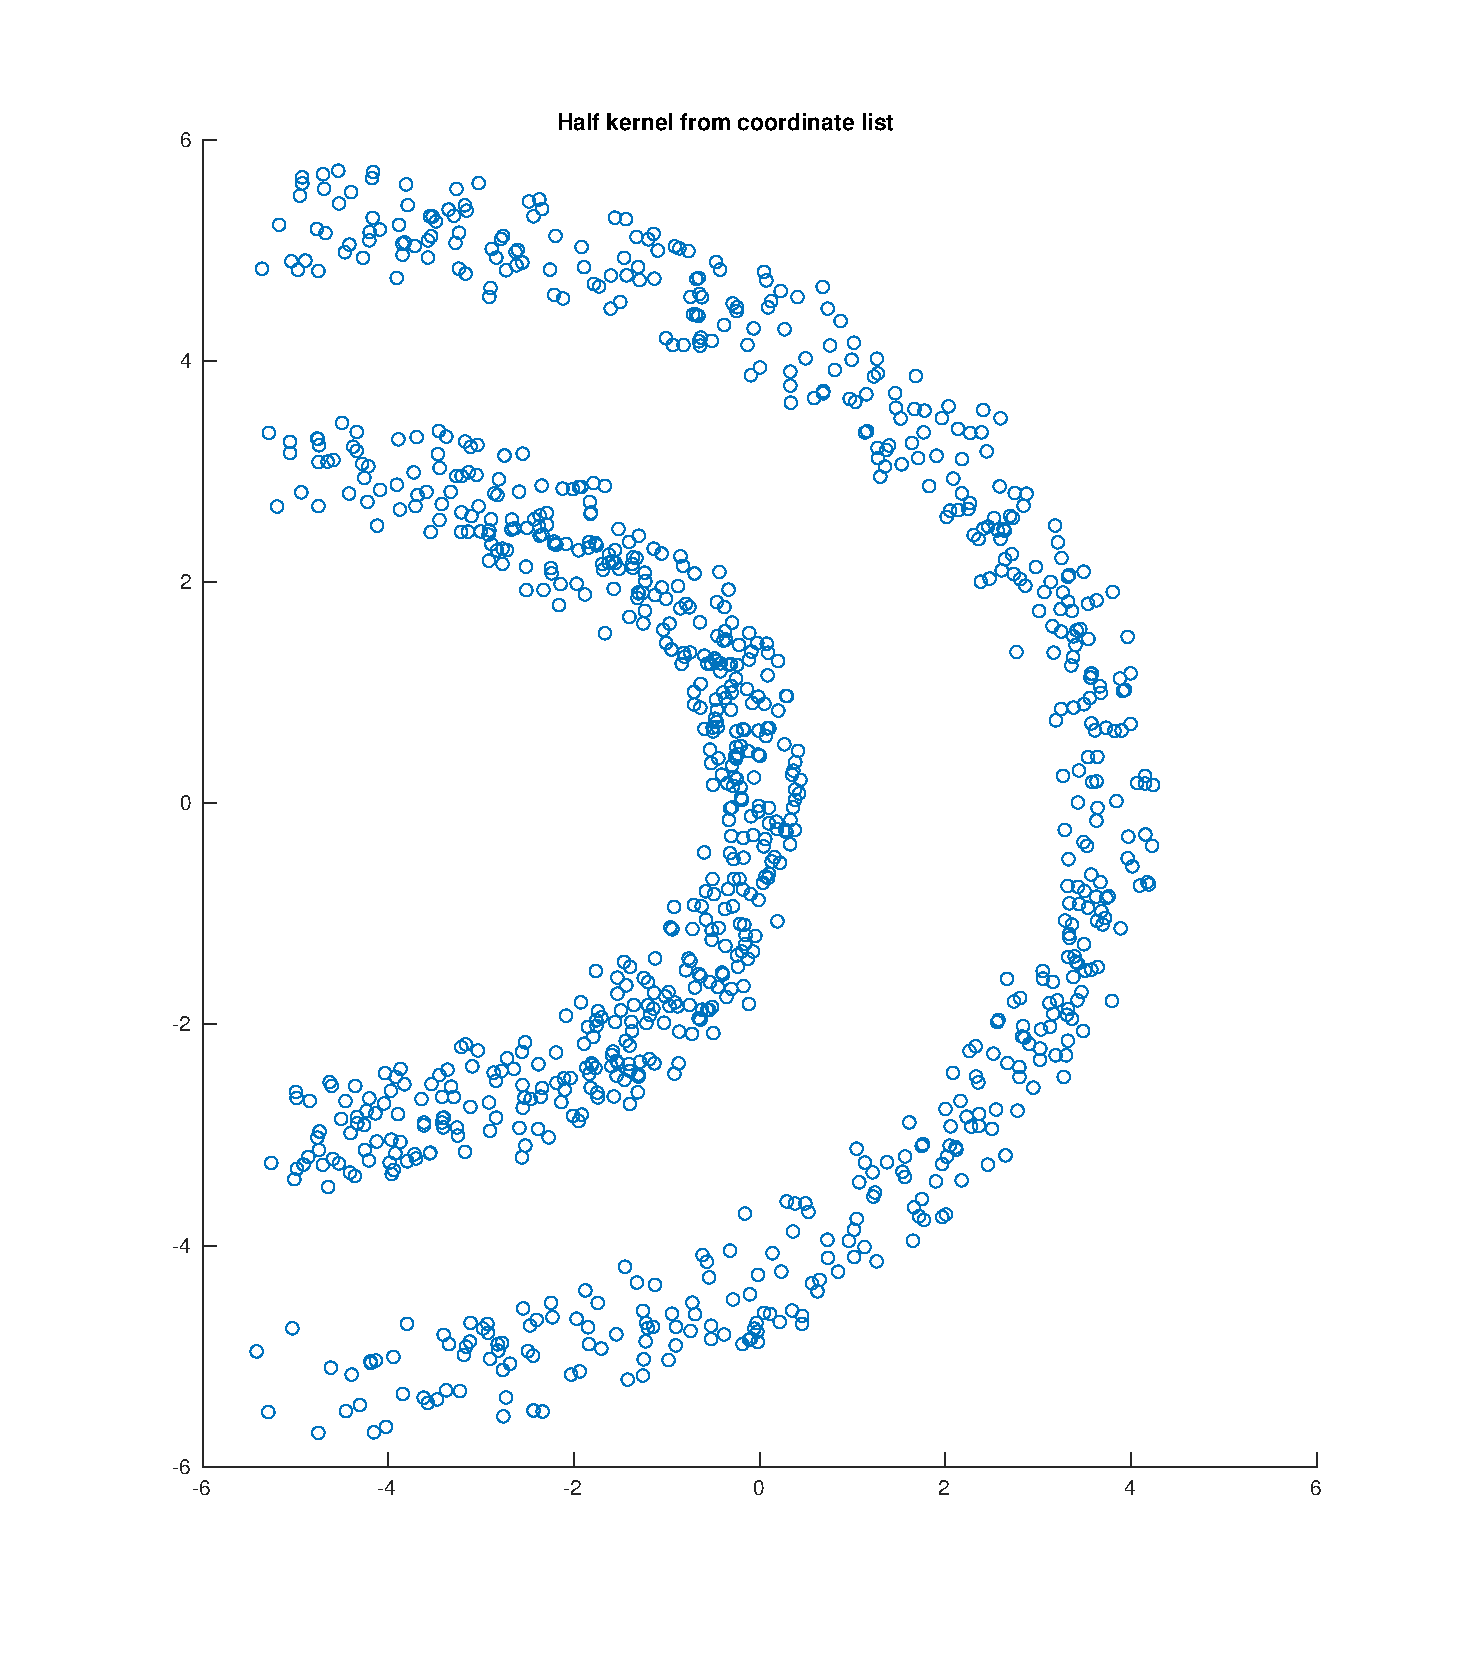
\includegraphics[width=.5\textwidth, trim={0cm 3cm 0cm 0cm}]{./img/ex1-1-halfkernel}
\end{figure}

The two obvious clusters are the two half circles shown in Figure \ref{fig:ex1-1-halfkernel}.\\
The difficulty of a clustering algorithm in this scenario, particularly the k-means clustering algorithm,
is that centroids would be in the upper and lower half of the graph,
and the clustering would assign points to the nearest centroids dividing the graph in half on line $y=0$.\\
Dividing the halfkernel with k-means for $K=2$ and make each semi circle be a cluster is unfeasable.

%--------------------------------------------------------------------------------------
\subsubsection{
    Find the minimal spanning tree of the full graph.
    Use this information to determine the $\epsilon$ factor for the $\epsilon$-similarity graph.}

\begin{lstlisting}[
        frame=single,
        numbers=left,
        style=Matlab-editor,
        basicstyle=\mlttfamily\small,
        label={lst:ex1-2-epsilonsimgraph},
        caption={$\epsilon$ neighboorhood graph function},
        captionpos=b]
mst = minSpanTree(S);
epsilon = max(mst, [], "all");
\end{lstlisting}
Generally, set $\epsilon$ to the length of the longest edge in the minimal spanning tree,
so the $\epsilon$ neighborhood graph is safely connected.\\
The heuristic followed to get $\epsilon$ in this case is: get matrix $S$ from the gaussian similarity function and
calculate the maximum largest element.
Thus, $\epsilon$ is directly influenced by $\sigma$.\\
It provide use with reasonably connected $\epsilon$ similarity graph due to the process
the gaussian similarity function does to generate $S$.
\[
    s(x_i, x_j) = e^{\frac{-||x_i - x_j||^2}{2\sigma^2}}
\]


%--------------------------------------------------------------------------------------
\subsubsection{
    Complete the Matlab function $epsilonSimGraph()$.
    It should generate the similarity matrix of the $\epsilon$-similarity graph.}

\begin{lstlisting}[
        frame=single,
        numbers=left,
        style=Matlab-editor,
        basicstyle=\mlttfamily\small,
        label={lst:ex1-3-epsilonsimgraph},
        caption={$\epsilon$ neighboorhood graph function},
        captionpos=b]
function [G] = epsilonSimGraph(epsilon,Pts)
    n = length(Pts);
    G = zeros(n, n);
    for i = 1:n
        for j = 1:n
            dist = norm(Pts(i,:) - Pts(j,:));
            if dist < epsilon
                G(i,j) = 1;
                G(j,i) = 1;
            end
        end
    end
end
\end{lstlisting}

In code snippet \ref{lst:ex1-3-epsilonsimgraph}, to create the $\epsilon$ neighboorhood graph function
connect all points whose pairwise distances are smaller than $\epsilon$.


%--------------------------------------------------------------------------------------
\subsubsection{
    Create the adjacency matrix for the $\epsilon$ similarity graph and
    visualize the resulting graph using the function $gplotg()$.}

\begin{lstlisting}[
        frame=single,
        numbers=left,
        style=Matlab-editor,
        basicstyle=\mlttfamily\small,
        label={lst:ex1-4-adjacency},
        caption={$\epsilon$ neighboorhood graph function},
        captionpos=b]
[G] = epsilonSimGraph(epsilon, Pts);
 W = S .* G;
gplotg(W, Pts(:,1:2));
title('Visualize adjacency matrix');
\end{lstlisting}

In code snippet \ref{lst:ex1-4-adjacency}, notice the element-wise multiplication
between the similarity matrix $S$ and the $\epsilon$ connectivity graph $G$.

%--------------------------------------------------------------------------------------
\subsubsection{
    Create the Laplacian matrix and implement spectral clustering.
    Your goal is to find the eigenvectors of the Laplacian corresponding to the $K = 2$ smallest eigenvalues.
    Afterwards, use the function $kmeans\_mod()$ to cluster the rows of these eigenvectors.}

\begin{lstlisting}[
        frame=single,
        numbers=left,
        style=Matlab-editor,
        basicstyle=\mlttfamily\small,
        label={lst:ex1-5-laplacian},
        caption={$\epsilon$ neighboorhood graph function},
        captionpos=b]
[L, ~] = CreateLapl(W);
[U, ~] = eigs(L, K, "smallestabs");
\end{lstlisting}

In code snippet \ref{lst:ex1-5-laplacian}, create the Laplacian matrix $L$ and
retrieve the first $K$ eigenvectors of $L$ as columns of matrix $U$ in ascending order.

%-- 1.6 ---------------------------------------------------------------------------------
\subsubsection{
    Use the $kmeans\_mod()$ function to perform k-means clustering on the input points.
    Visualize the two clustering results using the function $gplotmap()$.}

\begin{lstlisting}[
        frame=single,
        numbers=left,
        style=Matlab-editor,
        basicstyle=\mlttfamily\small,
        label={lst:ex1-6-kmeans},
        caption={$\epsilon$ neighboorhood graph function},
        captionpos=b]
[~, x_spec] = kmeans_mod(U, K, n);
[D_centroids_kmeans, x_kmeans] = kmeans_mod(Pts, K, n);
figure; gplotmap(W, Pts, x_spec); title('Spectral clusters')
figure; gplotmap(W, Pts, x_kmeans); title('K-means clusters')
\end{lstlisting}

In code snippet \ref{lst:ex1-6-kmeans}, cluster rows of eigenvector matrix of $L$
corresponding to $K$ smallest eigenvalues in U and get $x\_spec$, $x\_kmeans$ to plot the mappings using
adjacency graph $W$ and poits $Pts$.

%--------------------------------------------------------------------------------------
\subsubsection{Cluster the datasets: Two spirals, Cluster in cluster, Crescent \& full moon in $K = 2$ clusters,
    and visualize the results obtained with spectral clustering and k-means directly on the input data.
    Do the same for Corners, and Outlier for $K = 4$ clusters.
    Include the values of parameters $\epsilon, \sigma$}

A seed for the random number generator has been set $rng(20020309)$, for the results to be replicable.

Table \ref{table:ex1-7-coefficients} shows the values of $\epsilon$ and $\sigma$ used for each dataset.

\begin{table}[H]
    \centering
    \caption{Parameters $\epsilon, \sigma, K$ values}
    \label{table:ex1-7-coefficients}
    \begin{tabular}{||l l l l||}
        \hline
        Dataset               & $\sigma$ & $\epsilon$ & $K$ \\ [0.5ex]
        \hline\hline
        two spirals           & 7.600    & 0.687      & 2   \\
        cluster in cluster    & 6.919    & 0.632      & 2   \\
        crescent \& full moon & 7.389    & 0.595      & 2   \\
        corners               & 6.907    & 0.547      & 4   \\
        outlier               & 54.598   & 0.984      & 4   \\ [1ex]
        \hline
    \end{tabular}
\end{table}

\begin{figure}[H]
    \centering
    \caption{Two Spirals cluster, $K=2$}
    \label{fig:ex1-7-twospirals}
    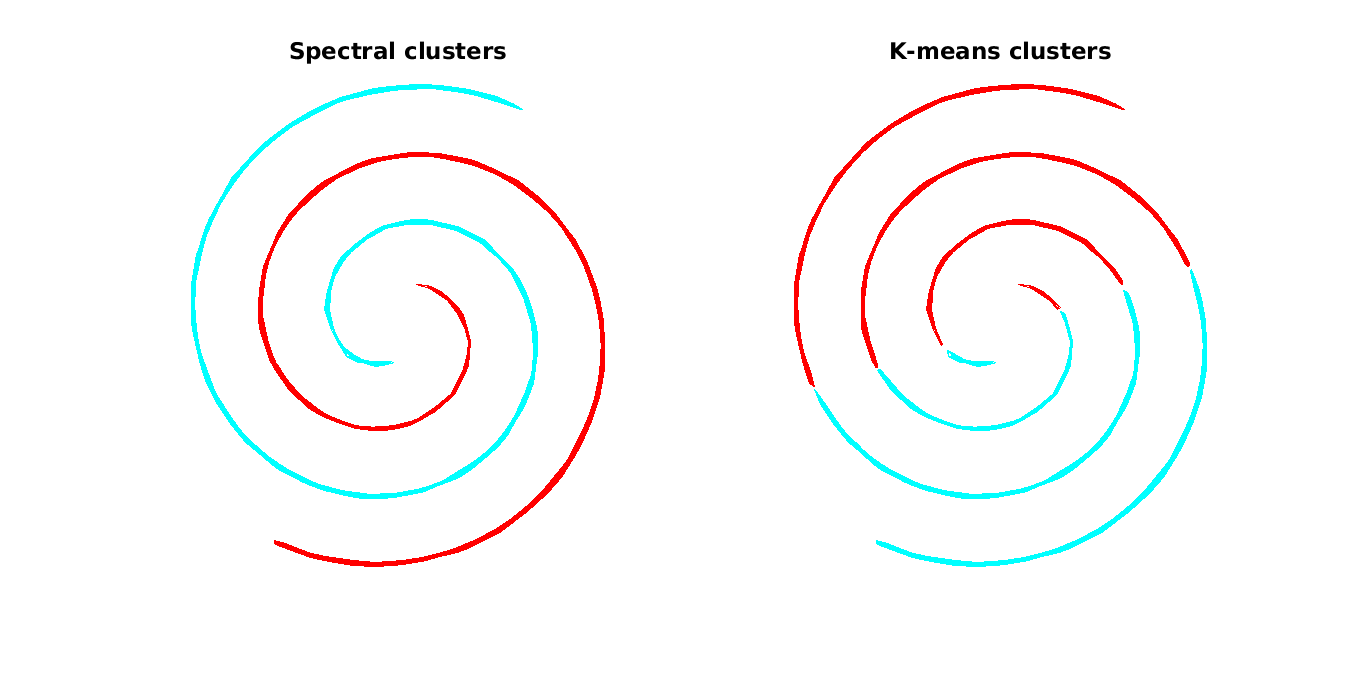
\includegraphics[width=\textwidth, trim={3cm 1cm 3cm 0cm}]{./img/ex1-7-twospirals.eps}
\end{figure}

Set $\sigma=log(n)$ by default.\\
Dataset \textit{twospirals} in Figure \ref{fig:ex1-7-twospirals} has its spectral clusters
assigning each cluster to a spiral, hence being visually logical.
The k-means clusters are instead divided diagonally with a clear line separating the two spirals
in half, not following the visually coordinate structured as spectral clustering.
Cetroids are placed in the middle of the cluster, hence one for each half of the graph.

\begin{figure}[H]
    \centering
    \caption{Cluster in Cluster cluster, $K=2$}
    \label{fig:ex1-7-clusterincluster}
    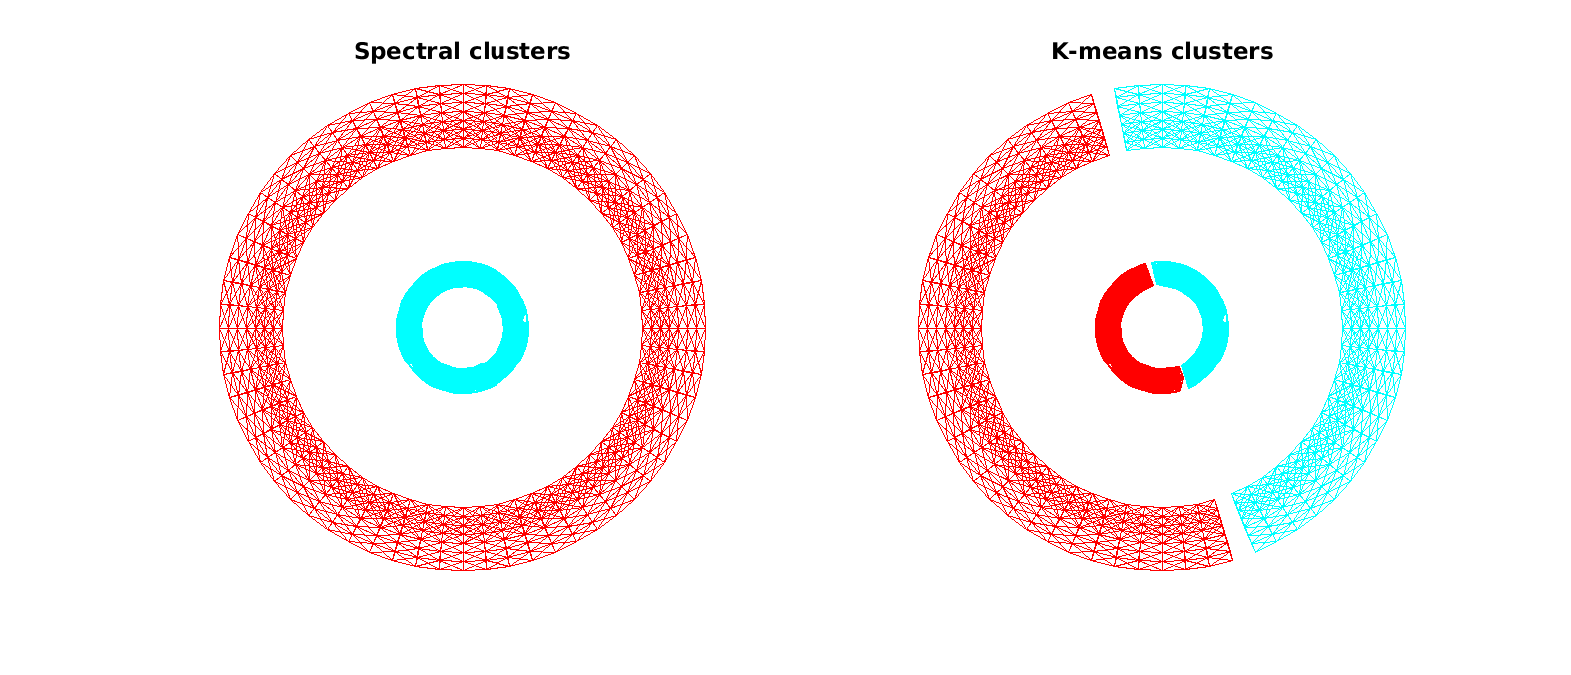
\includegraphics[width=\textwidth, trim={3cm 1cm 3cm 0cm}]{./img/ex1-7-clusterincluster.eps}
\end{figure}

Set $\sigma=log(n)$ by default.\\
Dataset \textit{clusterincluster} in Figure \ref{fig:ex1-7-clusterincluster} has its spectral clusters
assigning each cluster to its logical visual cluster representation.
The k-means clusters are instead dividing again the dataset with a clear line separating diagonally
in half the two nested clusters.
For both the inner cluster is colored denser because of the higher number of data points in the
inner cluster.
Again, blame the centroids.

\begin{figure}[H]
    \centering
    \caption{Crescent \& Full Moon cluster, $K=2$}
    \label{fig:ex1-7-crescentfullmoon}
    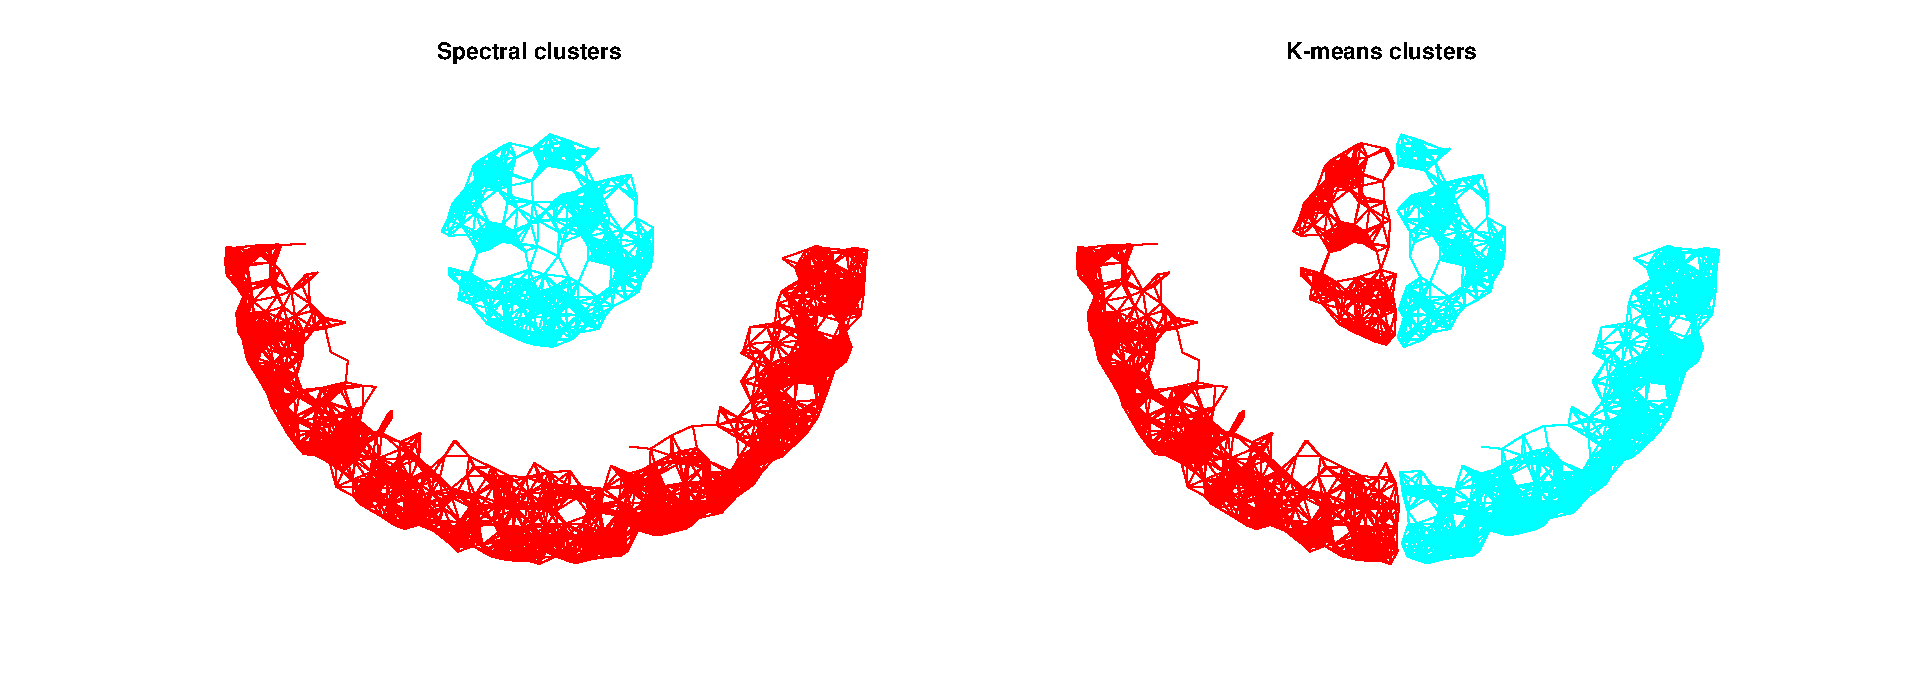
\includegraphics[width=\textwidth, trim={3cm 2cm 3cm 0cm}]{./img/ex1-7-crescentfullmoon.eps}
\end{figure}

Set $\sigma=exp(K)$ to increase the width of the neighboorhood connectivity and
make it dependent to the number of cluster $K$ and solve the ill conditioned problem.\\
Dataset \textit{crescentfullmoon} in Figure \ref{fig:ex1-7-crescentfullmoon} has its spectral clusters
assigning each data point to either the full moon of the crescent moon, hence being visually logical.
The k-means clusters are instead dividing again the dataset in half.
Again, blame the cetroids.

%--------------------------------------------------------------------------------------
\begin{figure}[H]
    \centering
    \caption{Corners cluster, $K=4$}
    \label{fig:ex1-7-corners}
    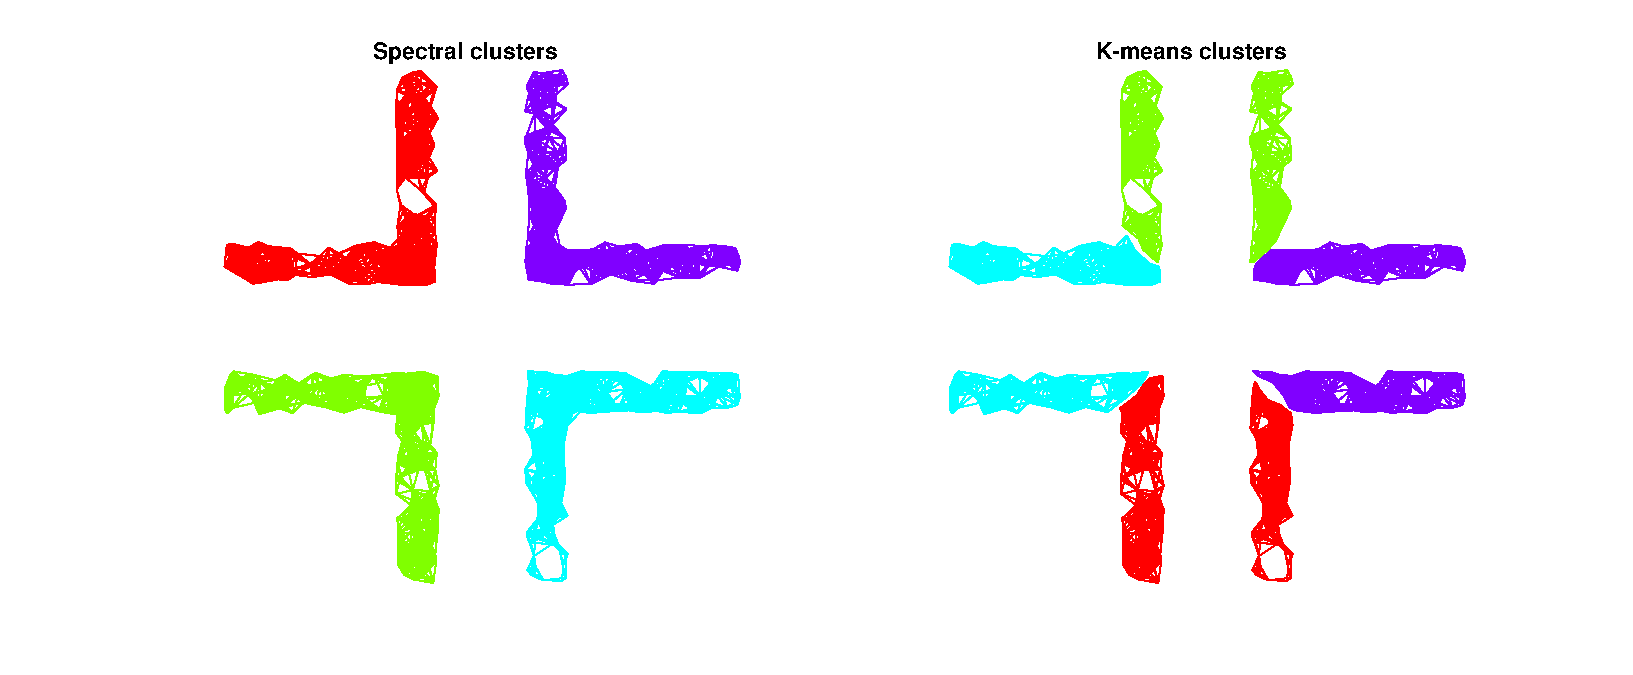
\includegraphics[width=\textwidth, trim={3cm 1cm 3cm 0cm}]{./img/ex1-7-corners.eps}
\end{figure}

Set $\sigma=log(n)$ by default.\\
Dataset \textit{corners} in Figure \ref{fig:ex1-7-corners} has its spectral clusters
assigning each data point to an "L" shaped figure cluster, hence being visually logical since the graph
is visually interconnected as this.
The k-means clusters are instead dividing each "L" shaped figure in half, with the centroids
placed between one "L" shaped figure and another, thus connecting near "L" shape halfs.

\begin{figure}[H]
    \centering
    \caption{Outlier cluster, $K=4$}
    \label{fig:ex1-7-outlier}
    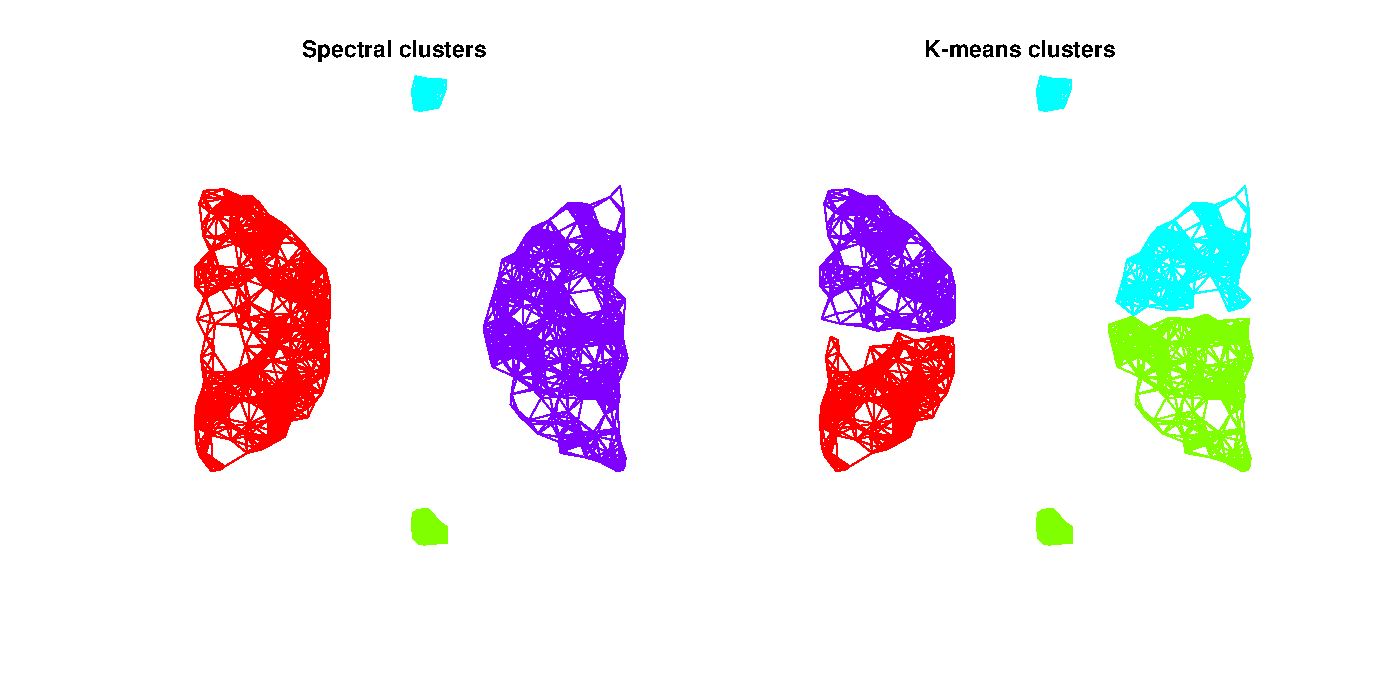
\includegraphics[width=\textwidth, trim={3cm 2cm 3cm 0cm}]{./img/ex1-7-outlier.eps}
\end{figure}

Set $\sigma=exp(K)$ to increase the width of the neighboorhood connectivity,
make it dependent to the number of cluster $K$ and solve the ill conditioned problem. \\
Dataset \textit{outlier} in Figure \ref{fig:ex1-7-outlier} has its spectral clusters
assigning each data point to an isolated group of the visually diveded 4 graph density agglomerates.
The k-means clusters are instead having trouble to find visually meaninful structure.

\cleardoublepage

% the larger sigma, the larger the area width of the neighboorhood

%--------------------------------------------------------------------------------------
\subsection{Spectral clustering of real-world graphs [35 points]}

All solutions provided from \textit{ClusterGraphs.m}, \textit{ClusterMetrics.m} source code.\\
A seed for the random number generator has been set $rng(20020309)$, for the results to be replicable.

%--------------------------------------------------------------------------------------
\subsubsection{
    Construct the Laplacian matrix, and draw the graphs using the eigenvectors to supply coordinates.
    Plot your results for all the three additionally supplied meshes: grid2, barth, 3elt.}

\begin{figure}[H]
    \centering
    \caption{Mesh airfoil1}
    \label{fig:ex2-1-airfoil1}
    \includegraphics[width=\textwidth, trim={4cm 1cm 4cm 0cm}]{./img/ex2-1-airfoil1.eps}
\end{figure}

\begin{figure}[H]
    \centering
    \caption{Mesh barth}
    \label{fig:ex2-1-barth}
    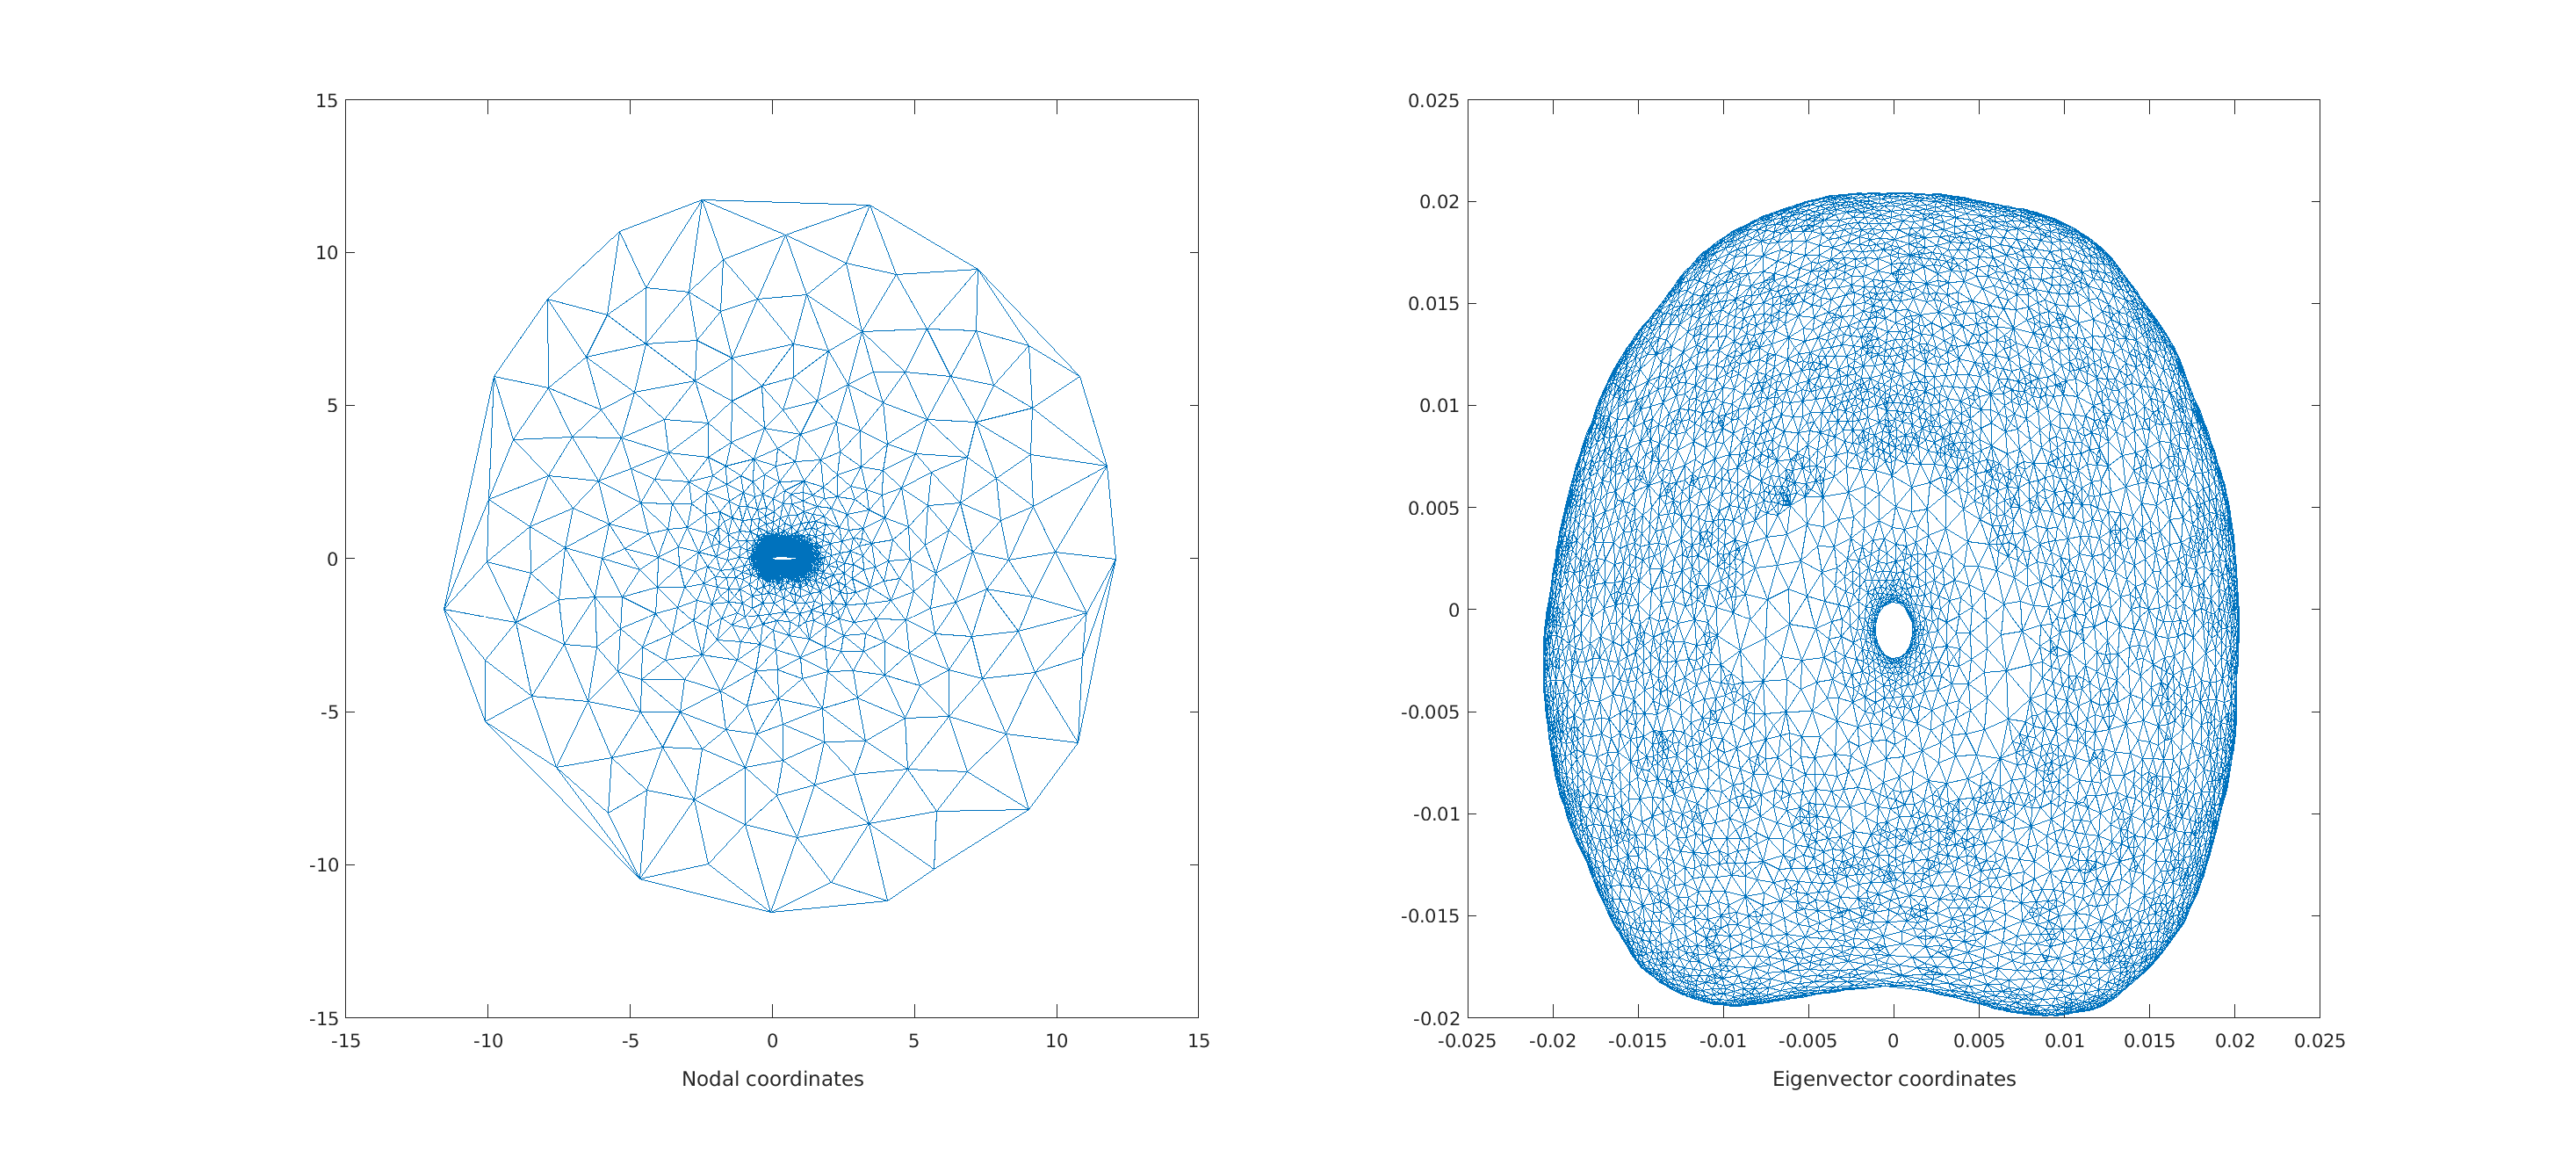
\includegraphics[width=\textwidth, trim={7cm 1cm 7cm 0cm}]{./img/ex2-1-barth.eps}
\end{figure}

\begin{figure}[H]
    \centering
    \caption{Mesh grid2}
    \label{fig:ex2-1-grid2}
    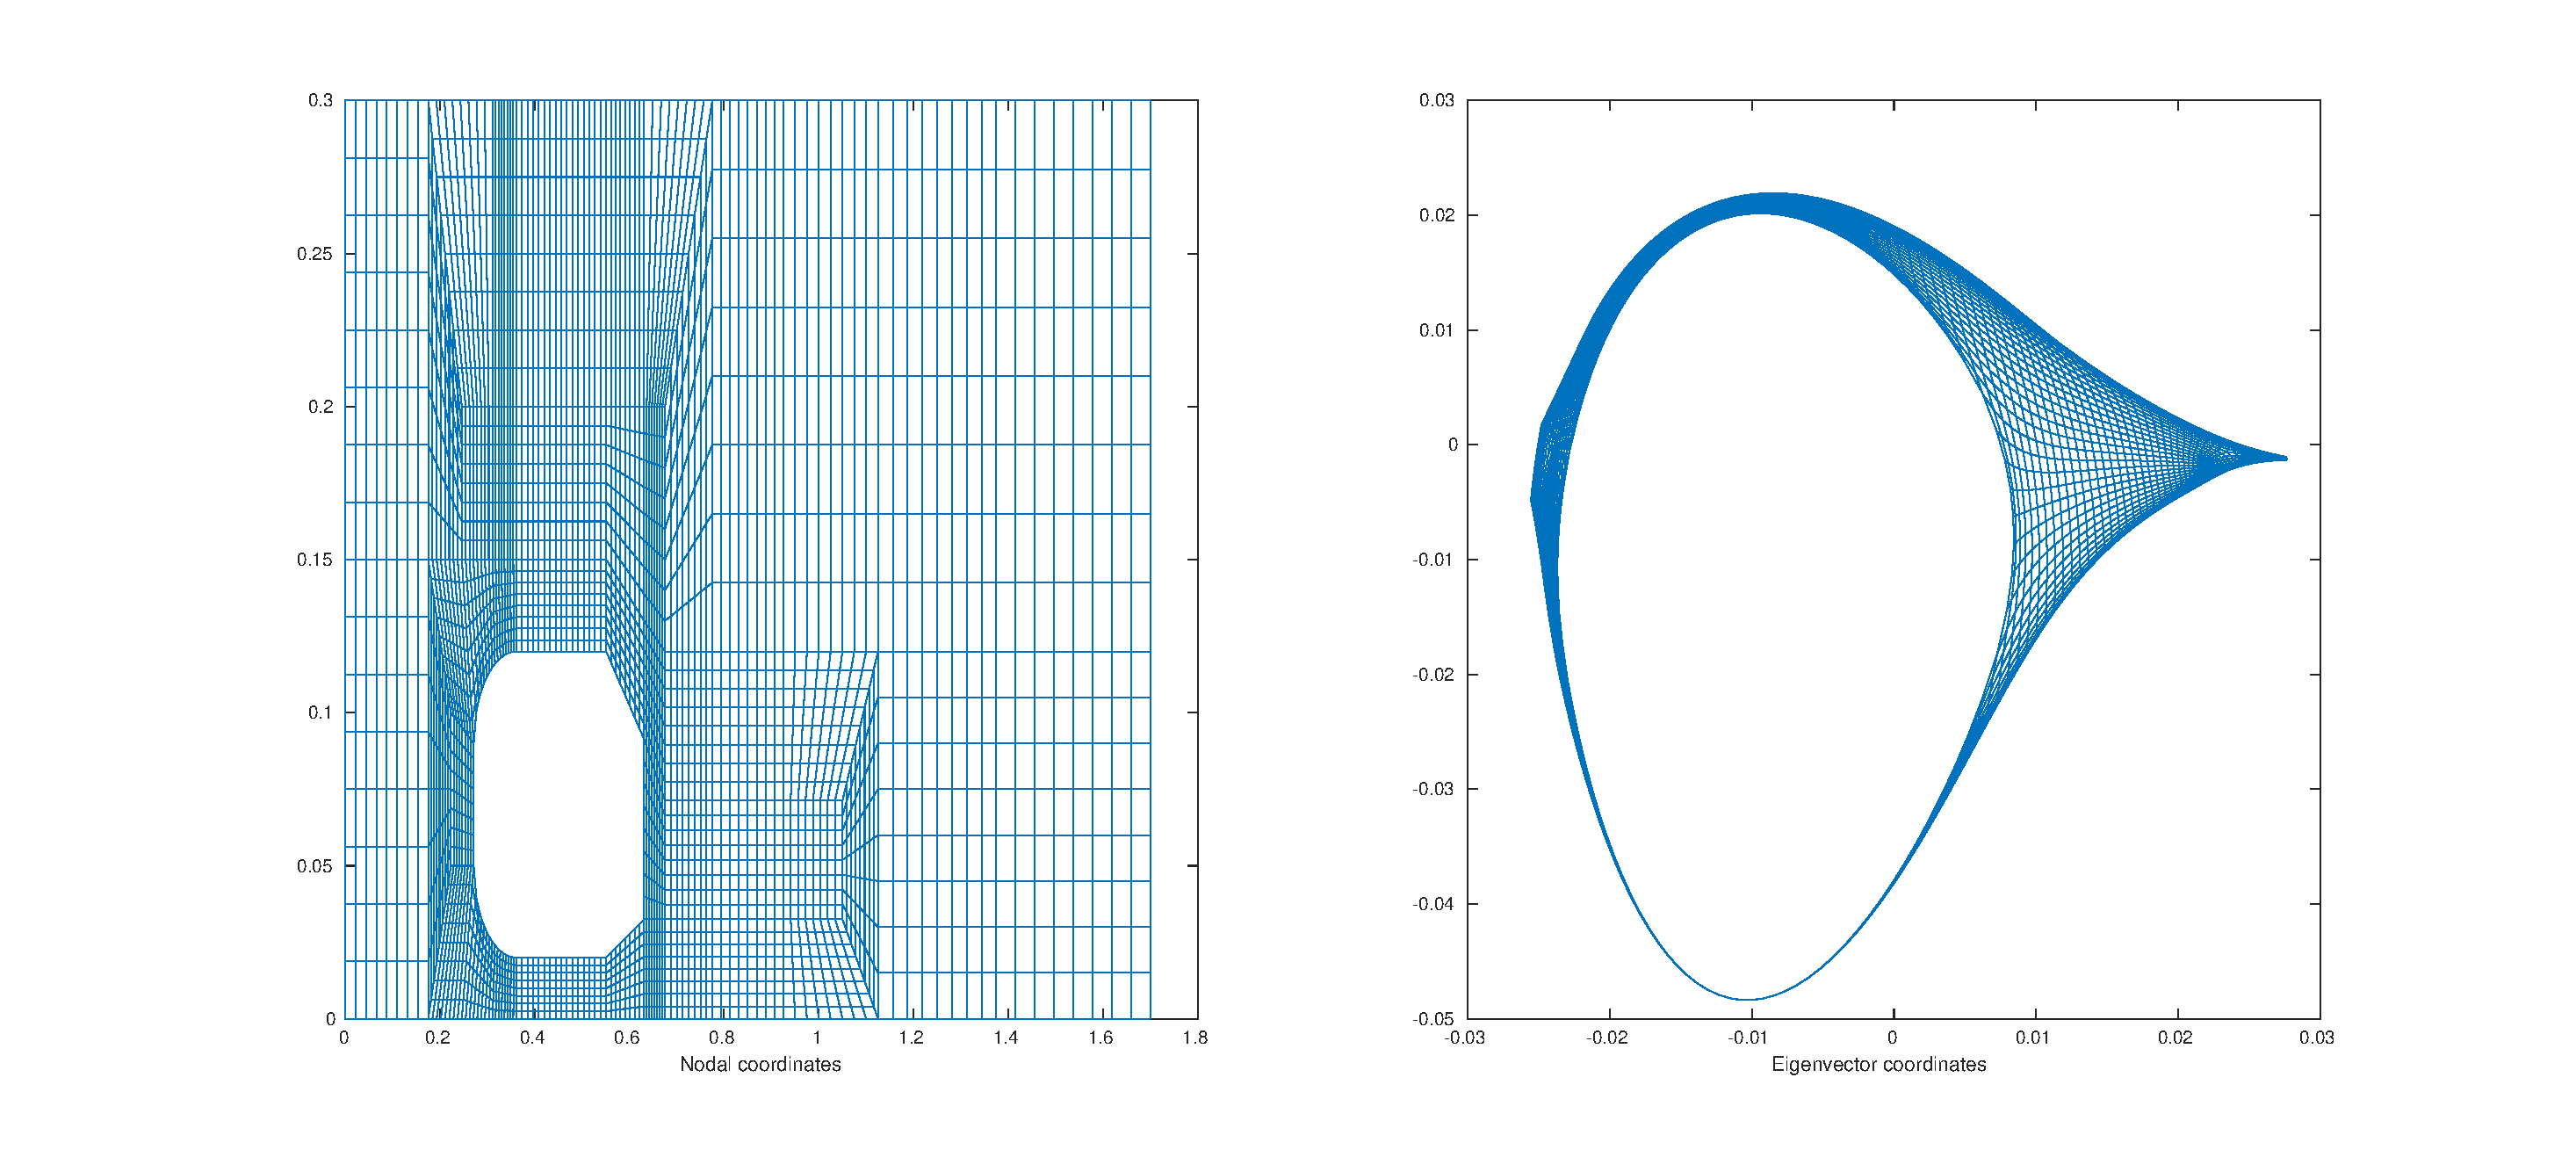
\includegraphics[width=\textwidth, trim={7cm 3cm 7cm 0cm}]{./img/ex2-1-grid2.eps}
\end{figure}

\begin{figure}[H]
    \centering
    \caption{Mesh 3elt}
    \label{fig:ex2-1-3elt}
    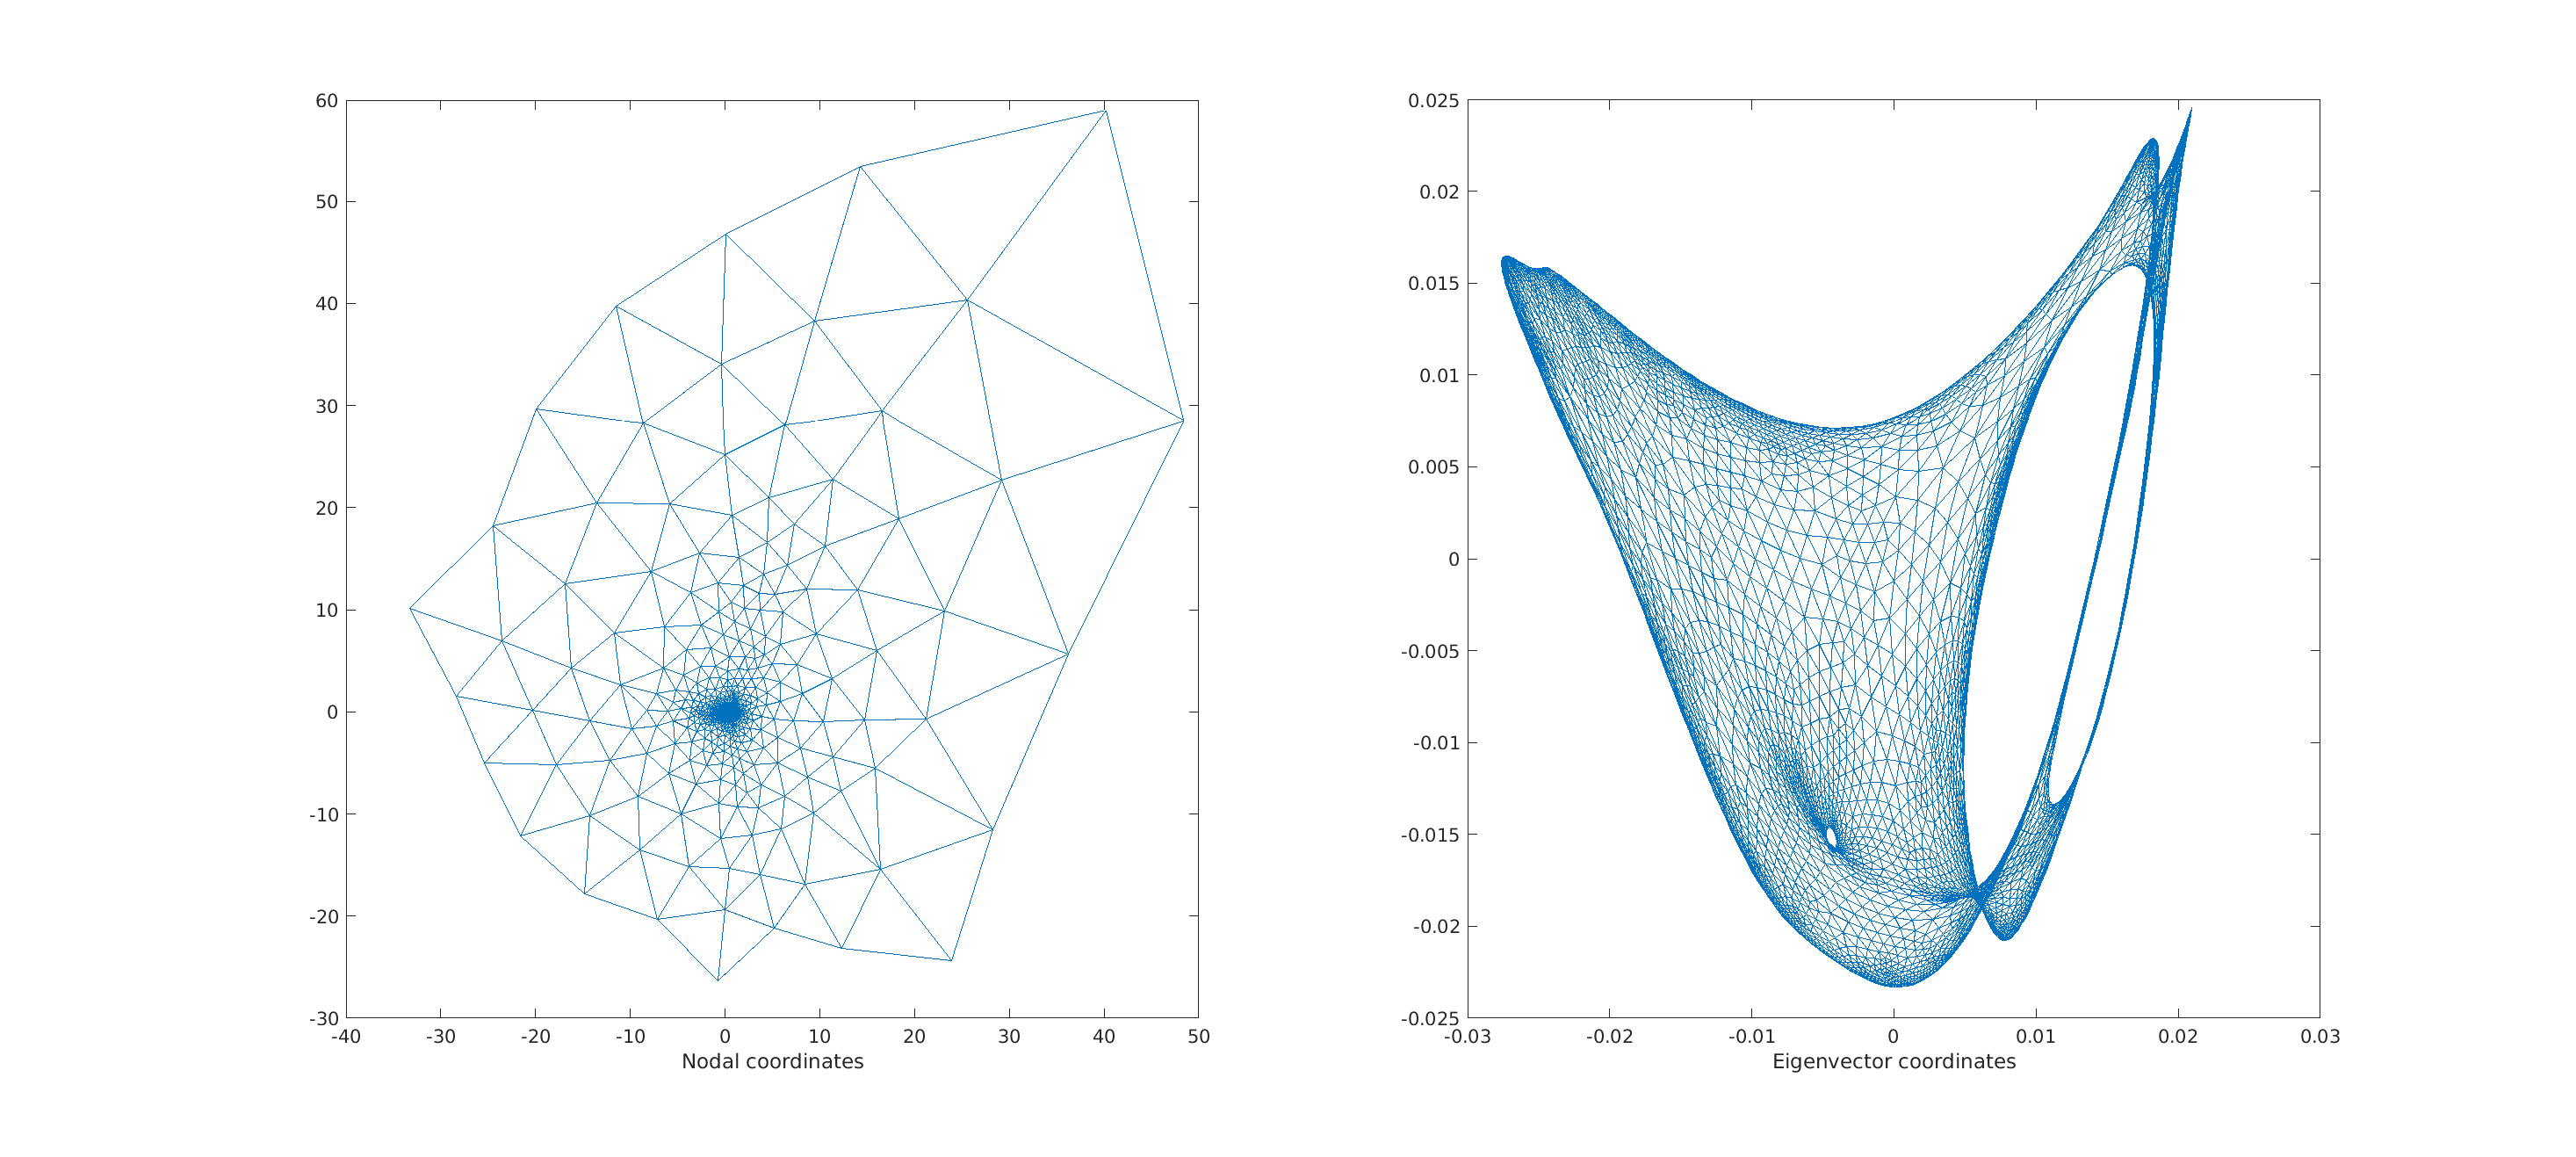
\includegraphics[width=\textwidth, trim={7cm 0cm 7cm 0cm}]{./img/ex2-1-3elt.eps}
\end{figure}

%--------------------------------------------------------------------------------------
\subsubsection{
    Cluster each graph in $K = 4$ clusters with the spectral and the k-means method.
    Plot all of your results and describe the differences that you can see
    in the output of the $2$ different algorithms and where they might come from.}

\begin{figure}[H]
    \centering
    \caption{Plot - Mesh airfoil1}
    \label{fig:ex2-2-airfoil1}
    \includegraphics[width=\textwidth, trim={0cm 5cm 0cm 0cm}]{./img/ex2-2-airfoil1.eps}
\end{figure}

\begin{figure}[H]
    \centering
    \caption{Plot eigvec coords - Mesh airfoil1 spectral clusters}
    \label{fig:ex2-2-airfoil1-eigs}
    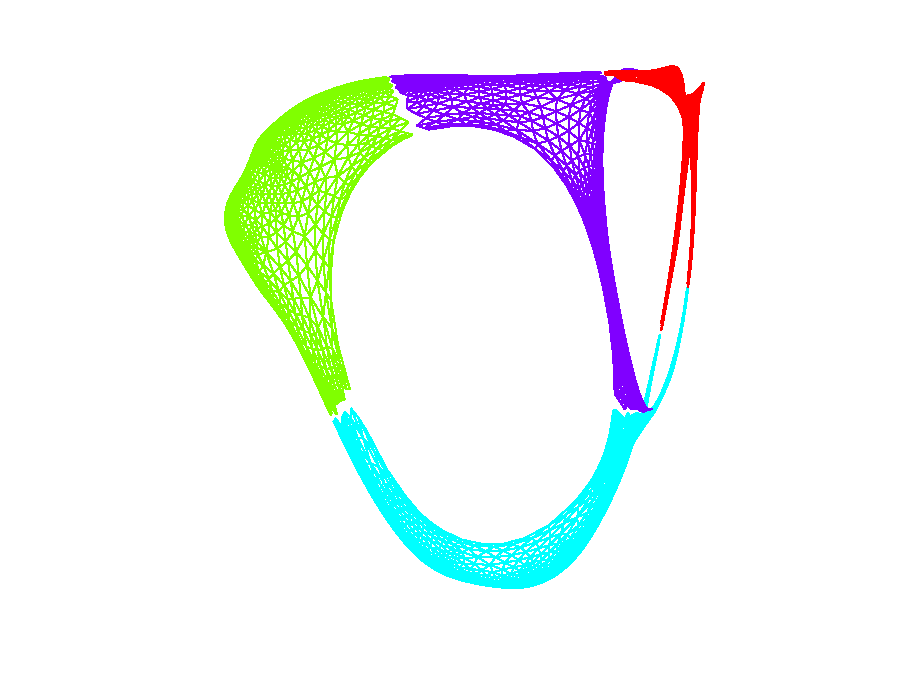
\includegraphics[width=\textwidth, trim={0cm 0cm 0cm 0.5cm}, clip]{./img/ex2-2-airfoil1-eigs.eps}
\end{figure}

Clustering for \textit{airfoil1} mesh in Figure \ref{fig:ex2-2-airfoil1}
Figure \ref{fig:ex2-2-airfoil1-eigs} show such reasoning.\\
The k-means clustering instead, gives a more pleasing visual result as the random nature of the
centroids position leverage such peculiarity.

\begin{figure}[H]
    \centering
    \caption{Plot - Mesh barth}
    \label{fig:ex2-2-barth}
    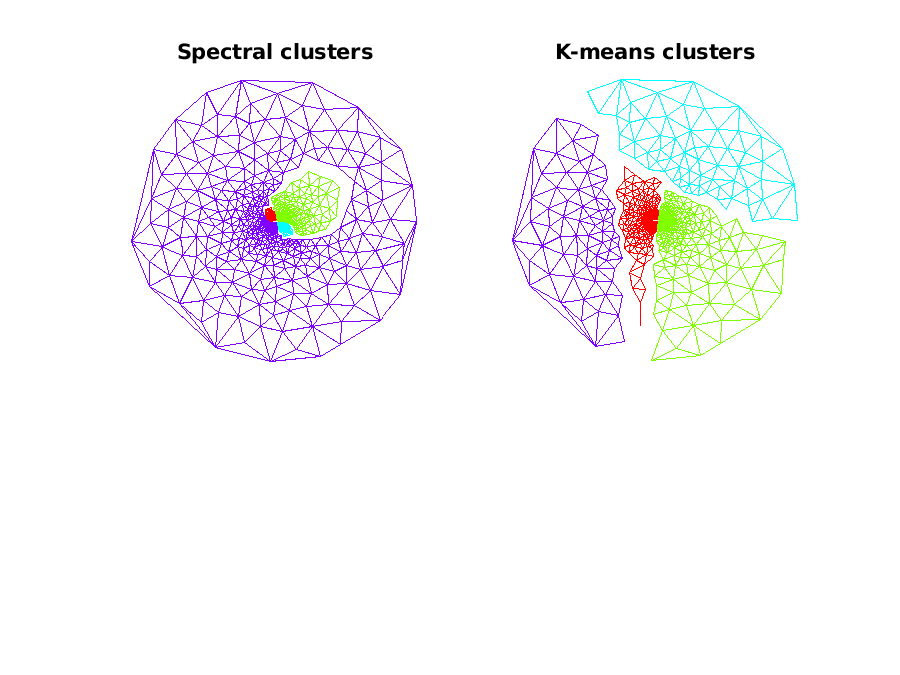
\includegraphics[width=\textwidth, trim={0cm 4.5cm 0cm 0cm}, clip]{./img/ex2-2-barth.eps}
\end{figure}

\begin{figure}[H]
    \centering
    \caption{Plot eigvec coords - Mesh barth spectral clusters}
    \label{fig:ex2-2-barth-eigs}
    \includegraphics[width=\textwidth, trim={0cm 0cm 0cm 0.5cm}, clip]{./img/ex2-2-barth-eigs.eps}
\end{figure}

Clustering for \textit{barth} mesh in Figure \ref{fig:ex2-2-barth} presents some particurality:
the spectral clustering considers the graph density as in Figure \ref{fig:ex2-1-barth},
which is really high at the center of the mesh,
hence, though we hardly see the 4 clusters,
they are balanced divided in density in comparison with one another.
Figure \ref{fig:ex2-2-barth-eigs} show such reasoning.\\
The k-means clustering instead, gives a more pleasing visual result as the random nature of the
centroids position leverage such peculiarity.

\begin{figure}[H]
    \centering
    \caption{Plot - Mesh grid2}
    \label{fig:ex2-2-grid2}
    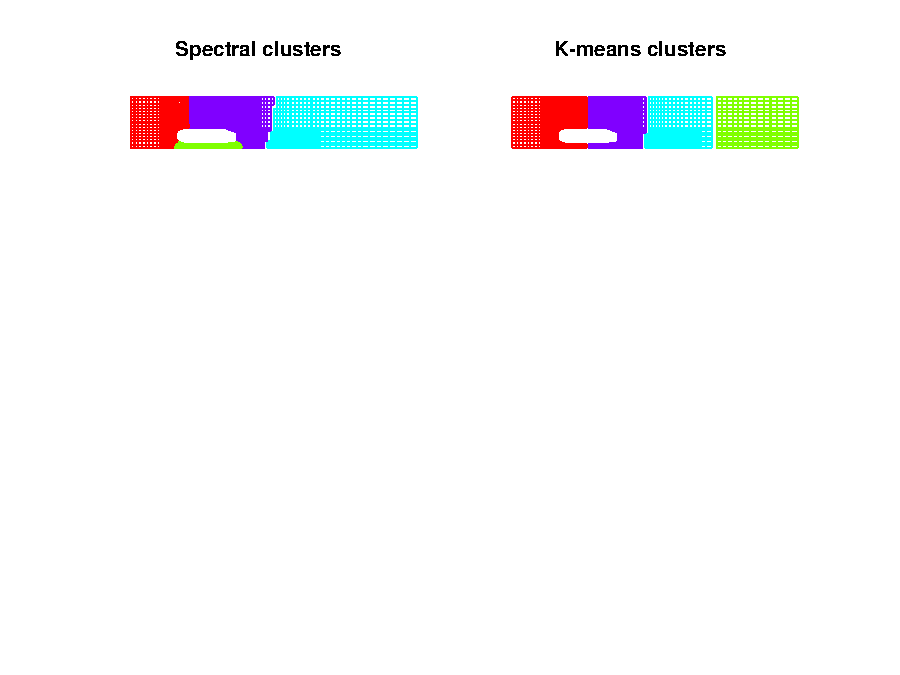
\includegraphics[width=\textwidth, trim={0cm 8cm 0cm 0cm}, clip]{./img/ex2-2-grid2.eps}
\end{figure}

\begin{figure}[H]
    \centering
    \caption{Plot eigvec coords - Mesh grid2 spectral clusters}
    \label{fig:ex2-2-grid2-eigs}
    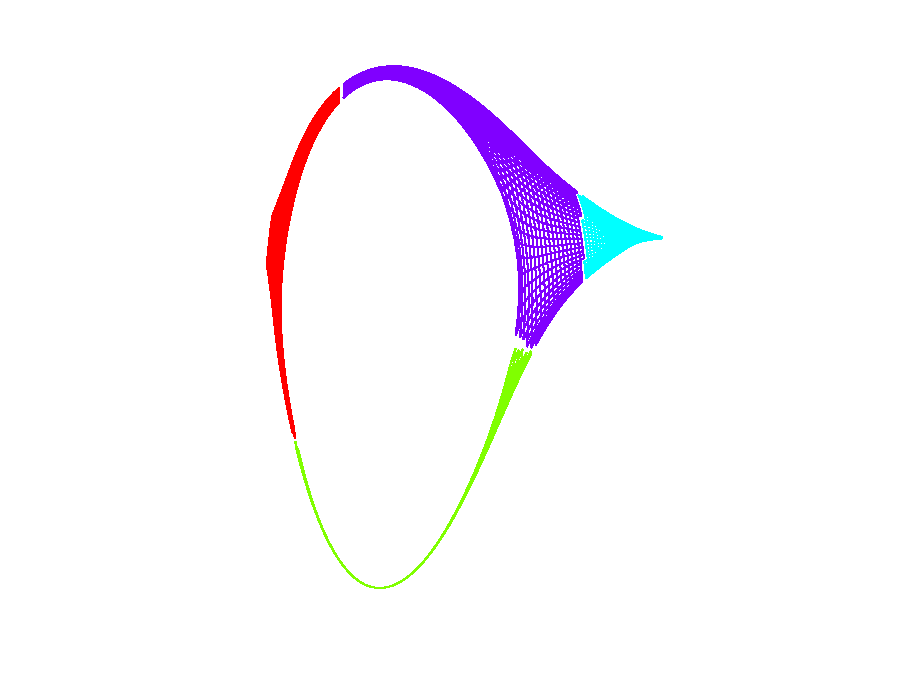
\includegraphics[width=\textwidth, trim={0cm 1cm 0cm 0.5cm}, clip]{./img/ex2-2-grid2-eigs.eps}
\end{figure}

Clustering for the \textit{grid2} mesh in Figure \ref{fig:ex2-2-grid2} is the most visully balanced
of all the meshes provided:
that is visually inferrable from its nodal coordinates in Figure \ref{fig:ex2-1-grid2}
that k-means clustering take in consideration, hence its geometrical distance.\\
The spectral clustering have the peculiarity of marking the right large area of graph
as a single cluster and the base under the "bridge" as another one, which is again derived and visible
from the structure of the plotted graph using its eigenvector coordinates in Figure \ref{fig:ex2-1-grid2}.

\begin{figure}[H]
    \centering
    \caption{Plot - Mesh 3elt}
    \label{fig:ex2-2-3elt}
    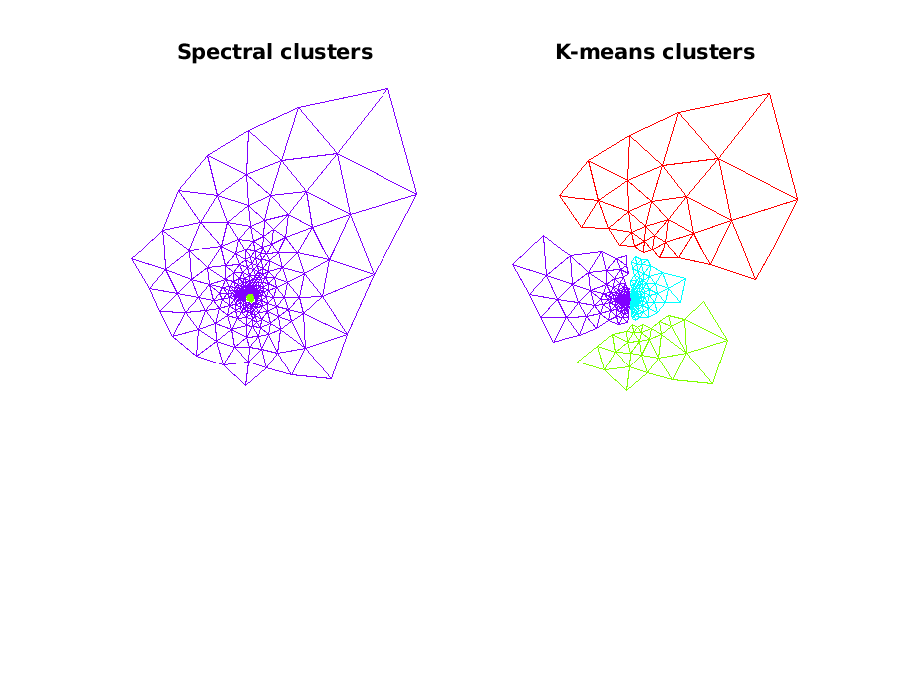
\includegraphics[width=\textwidth, trim={0cm 4.5cm 0cm 0cm}, clip]{./img/ex2-2-3elt.eps}
\end{figure}

\begin{figure}[H]
    \centering
    \caption{Plot eigvec coords - Mesh 3elt spectral clusters}
    \label{fig:ex2-2-3elt-eigs}
    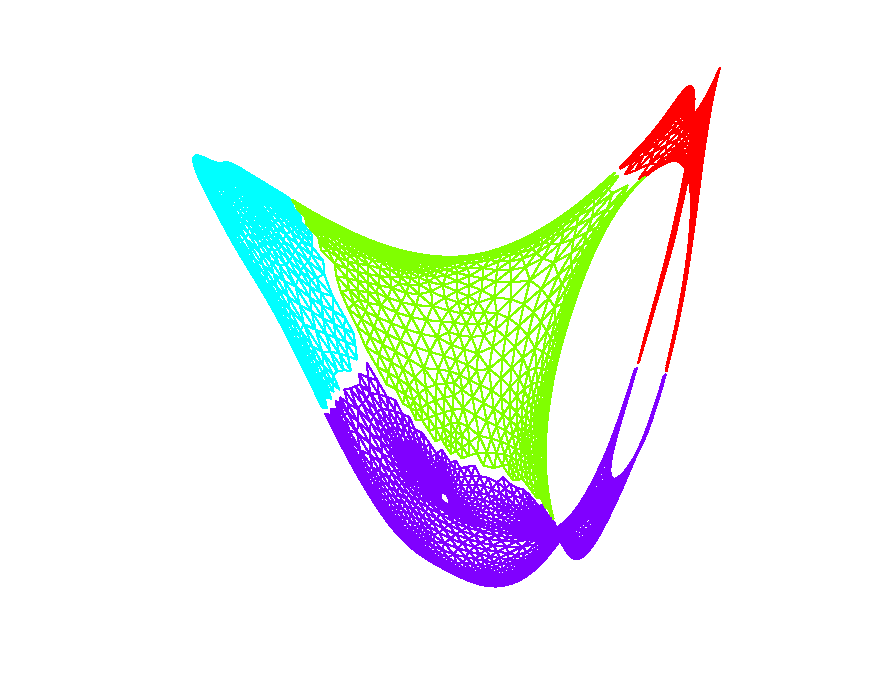
\includegraphics[width=\textwidth, trim={0cm 1cm 0cm 1cm}, clip]{./img/ex2-2-3elt-eigs.eps}
\end{figure}

Clustering for the \textit{3elt} mesh in Figure \ref{fig:ex2-2-3elt} has the spectral clustering
presenting the most visually non intuitive clustering: there are 4 clusters but they are almost inexistent
visually, with one outer cluster predominating and another in the center of the graph with the other 2
not visible from the plot.
This phenomenon is explainable again by looking at the eigenvector coordinates plot
in Figure \ref{fig:ex2-1-3elt} as the mesh is highly dense in the center while the outer part is
almost visually sparse.
\\

%--------------------------------------------------------------------------------------
\subsubsection{
    Report in Table \ref{table:ex2-3-table}
    the number of nodes per cluster and plot a histogram of the reported values.
    What can you observe?}

A seed for the random number generator has been set $rng(20020309)$, for the results to be replicable.

\begin{table}[H]
    \centering
    \caption{Clustering results, $K = 4$}
    \label{table:ex2-3-table}
    \begin{tabular}{l|l|l}
        Case     & Spectral               & K-Means              \\
        \hline
        airfoil1 & 1150, 1050, 971, 1082  & 1846, 1292, 412, 703 \\
        grid2    & 785, 1305, 827, 379    & 604, 1183, 1271, 238 \\
        barth    & 1407, 2206, 1490, 1588 & 65, 71, 3884, 2671   \\
        3elt     & 874, 1794, 965, 1087   & 3098, 1560, 31, 31   \\
    \end{tabular}
\end{table}

%--- grid2 --------------------------------------------------------------------------------
\begin{figure}[H]
    \centering
    \caption{airfoil1 histogram - nodes per cluster}
    \label{fig:ex2-3-airfoil1}
    \includegraphics[width=\textwidth, trim={0cm 0cm 0cm 0cm}, clip]{./img/ex2-3-airfoil1.eps}
\end{figure}


%--- grid2 --------------------------------------------------------------------------------
\begin{figure}[H]
    \centering
    \caption{grid2 histogram - nodes per cluster}
    \label{fig:ex2-3-grid2}
    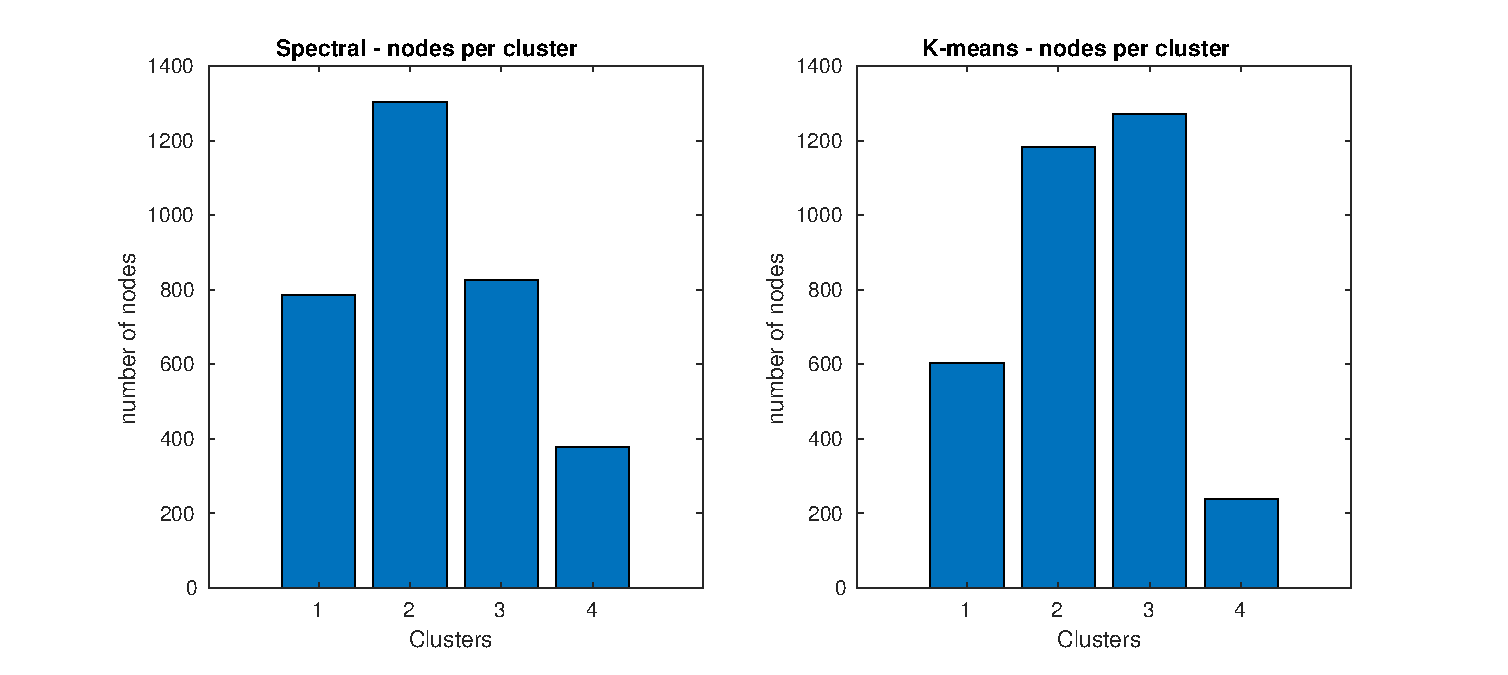
\includegraphics[width=\textwidth, trim={0cm 0cm 0cm 0cm}, clip]{./img/ex2-3-grid2.eps}
\end{figure}

In Figure \ref{fig:ex2-3-grid2}, both the clustering algorithms are presenting unbalanced clusters, with the  k-means clustering
presenting the maximum difference in number of nodes between the clusters: \\
k-means: $max \# nodes - min \# nodes = 1271 - 238 = 1033$\\
spectral: $max \# nodes - min \# nodes = 1305 - 379 = 926$\\
Such result from k-means is what we expected, though the difference in number of nodes is
generally expected to be lower on the spectral clustering algorithm since is known for its
stable and diffuse cluster results.

%--- barth --------------------------------------------------------------------------------
\begin{figure}[H]
    \centering
    \caption{barth histogram - nodes per cluster}
    \label{fig:ex2-3-barth}
    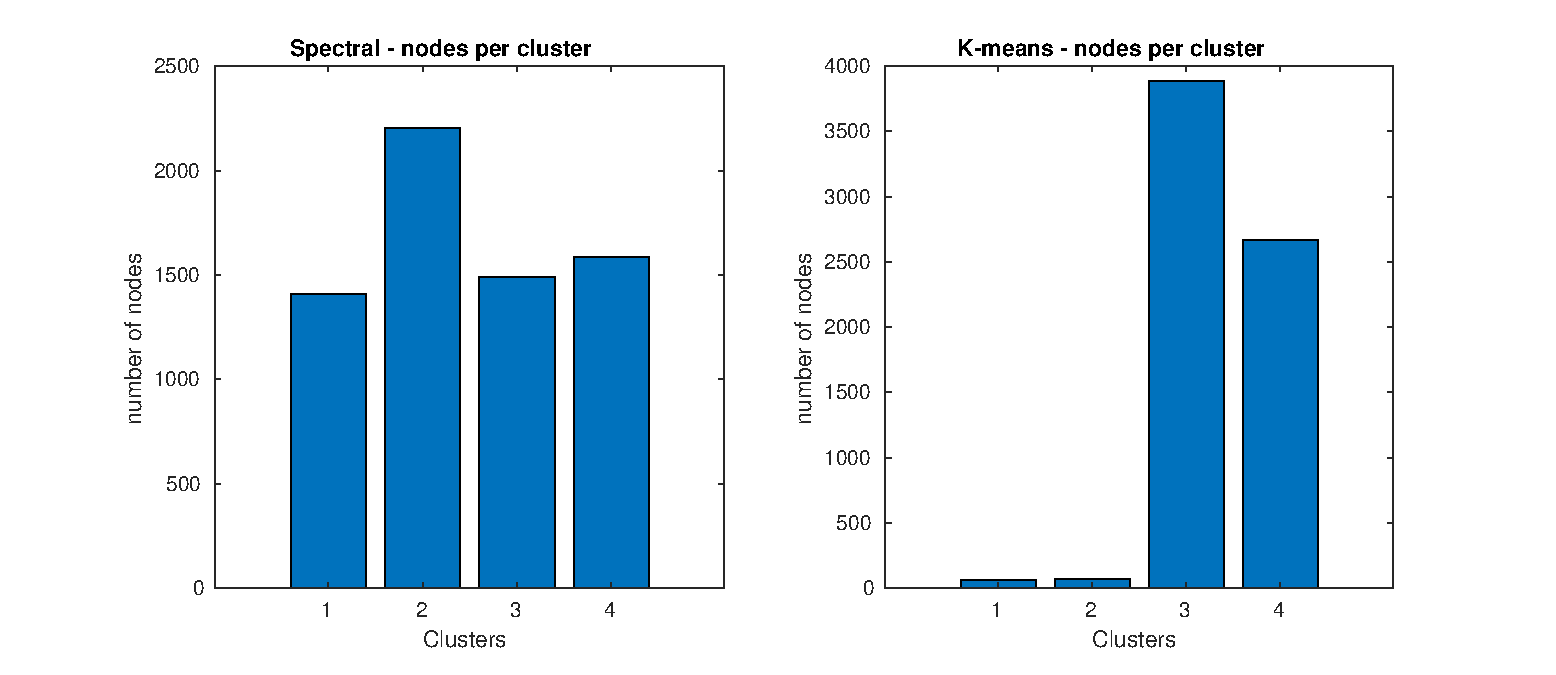
\includegraphics[width=\textwidth, trim={0cm 0cm 0cm 0cm}, clip]{./img/ex2-3-barth.eps}
\end{figure}

In Figure \ref{fig:ex2-3-barth}, the stability expected from the spectral clustering algorithm
is met and the clusters for this example are the most balanced of all the meshes provided.
Instead, the k-means clustering algorithm is clearly presenting a discrepancy in balance of number of nodes
per cluster, with the first 2 having very few almost neglectible number of nodes
and the last 2 comprending most of them.

%--- 3elt --------------------------------------------------------------------------------
\begin{figure}[H]
    \centering
    \caption{3elt histogram - nodes per cluster}
    \label{fig:ex2-3-3elt}
    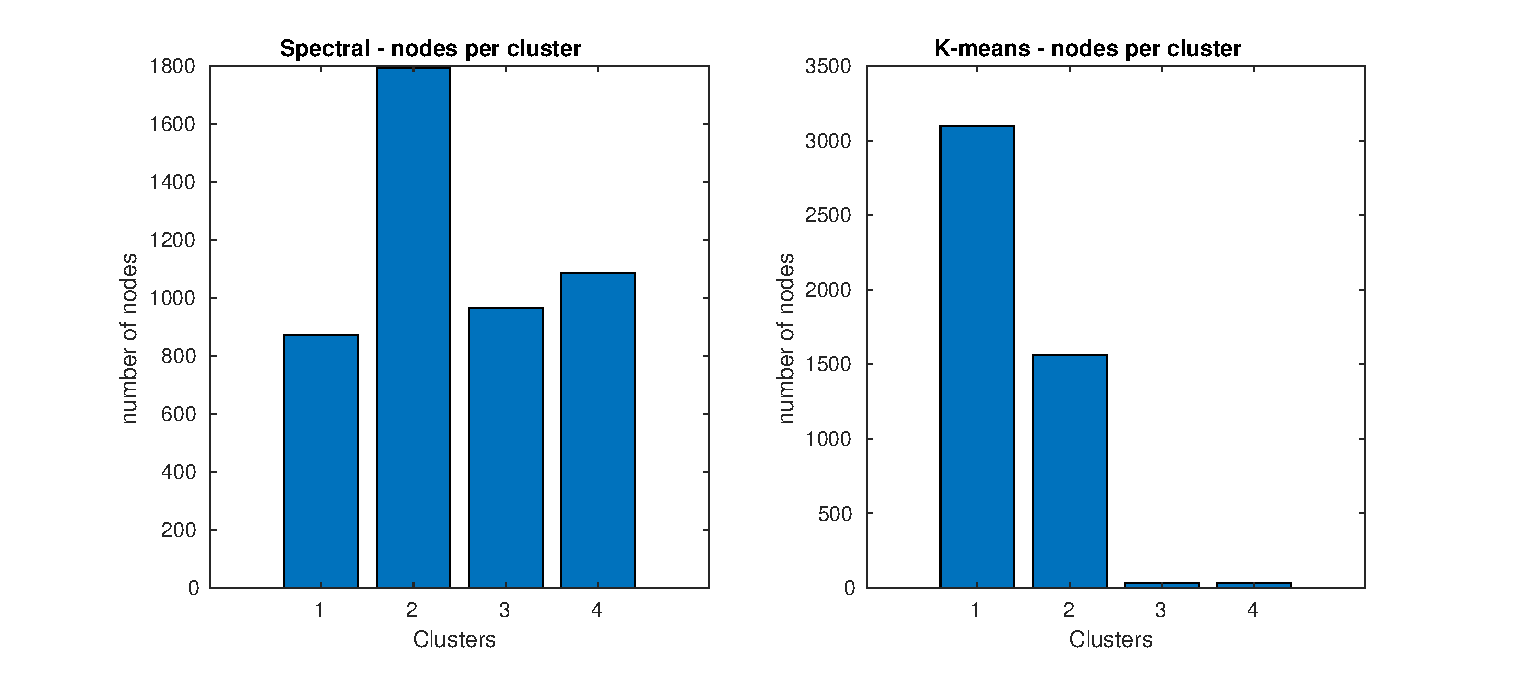
\includegraphics[width=\textwidth, trim={0cm 0cm 0cm 0cm}, clip]{./img/ex2-3-3elt.eps}
\end{figure}

In Figure \ref{fig:ex2-3-3elt}, the stability and balance expected from the spectral clustering algorithm
holds with only cluster \#2 being an bit of an exception.
Instead, the k-means clustering algorithm is again presenting an evident discrepancy in balance of number of nodes
per cluster.

\end{document}
